\scanpage{4}

\diagram{\begin{tikzcd}[ampersand replacement=\&,column sep=.8em,row sep=1.2ex]
\mathrm{Ob}\,C_4 \&
{\tikz[x=.008cm,y=-.008cm,baseline=-.3ex,line cap=round,line join=round]{
% The secure right-pointing arrow and its finer retracing are traced literally.
% Uncertain writing history: a separate cancelled left arrow is not established.
\draw[line width=.85pt] (606,136)..controls(736,145)and(900,178)..(1028,177);
\draw[line width=.35pt] (612,161)..controls(687,118)and(820,140)..(1009,174)
 (671,143)..controls(802,139)and(890,169)..(1025,177)
 (836,168)--(864,187) (606,137)--(616,146)
 (821,166)..controls(900,184)and(986,186)..(1024,177);
\draw[line width=.85pt] (999,152)--(1028,177)--(965,203)
 (1006,161)--(1028,177)--(986,190);
}} \& \mathrm{Fl}_0(\unsure{\ell_n|C_n|\ell_1|C_1})\\
{\bigl(\tikz[baseline=(topF.base)]{\node[inner sep=0pt] (topF) {\(\mathbb F\)};
% Detached ink fleck below and right of F; its linguistic status is uncertain.
\fill ([xshift=.08em,yshift=-.08em]topF.south east) circle[radius=.24pt];}
\mathrm l\,C_1\times\mathrm{Ob}\,C_2\bigr)}
 \arrow[u,shift left=.55ex]\arrow[u,shift right=.55ex]
 \& {\begin{gathered}
 \deleted{\amalg}\;\deleted{\unsure{\mathrm{Fl}_0 C_1\times}}\\[-.3ex]
 \inserted{\mathbb F\mathrm l_0(\unsure{\ell_1|C_1})\times\mathrm{Ob}\,C_2}
 \end{gathered}} \&
\end{tikzcd}}

\[
\mathbb F\mathrm l\,C_{\deleted{\unsure{2}}\unsure{1|2}}\times
\mathbb F\mathrm l(C_2)\times\deleted{\unsure{\mathrm{Fl}}}\mathrm{Ob}\,C_3
\]

\figure{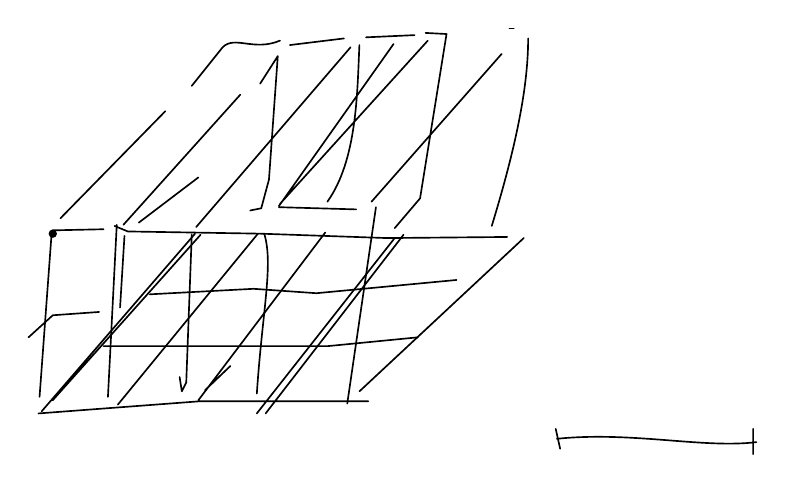
\begin{tikzpicture}[x=.014cm,y=-.014cm,line width=.6pt,line cap=round,line join=round]
\draw (1305,284)--(1351,283) (1361,280)--(1373,285)--(1493,287)--(1608,291)--(1717,290)
 (1304,286)--(1293,435) (1363,279)--(1355,435) (1370,289)--(1366,354)
 (1431,288)--(1426,422)--(1422,430)--(1420,417)
 (1497,288)..controls(1505,316)and(1495,357)..(1490,432) (1598,263)--(1572,441);
\draw (1292,450)--(1438,439)--(1591,439)
 (1295,448)--(1434,287) (1305,438)--(1439,288)
 (1364,442)--(1491,287) (1437,438)--(1552,286) (1443,429)--(1466,407)
 (1490,450)--(1615,291) (1498,450)--(1623,288) (1583,430)--(1732,291);
\draw (1283,381)--(1305,361)--(1347,358) (1351,389)--(1554,389)--(1636,381)
 (1393,342)--(1487,337)--(1544,341)--(1671,329);
\draw (1312,273)--(1407,176) (1369,279)--(1475,161) (1383,277)--(1437,236)
 (1431,153)--(1459,118)..controls(1470,107)and(1487,122)..(1511,112)
 (1493,151)--(1509,126)--(1501,238)--(1494,264)--(1484,266)
 (1520,116)--(1569,110) (1435,281)--(1575,118)
 (1510,262)--(1614,115) (1510,263)--(1580,265)
 (1554,258)..controls(1581,220)and(1581,159)..(1583,116)
 (1589,109)--(1633,107) (1511,260)--(1645,112)
 (1643,105)--(1662,106)--(1638,255)--(1615,282)
 (1594,258)--(1712,124) (1703,280)..controls(1725,208)and(1736,154)..(1736,110);
\fill (1305,287) circle[radius=3.8];
\draw (1719,101)--(1723,101); % detached short mark above the upper-right side
\draw (1762,473)..controls(1830,466)and(1895,482)..(1943,476)
 (1761,464)--(1765,482) (1940,464)--(1940,487);
\end{tikzpicture}}

\[
\mathbb F_3=\mathrm{Fl}\,C_1\times\mathrm{Fl}\,C_2
\,<\,\mathrm{Fl}\,\unsure{l_3|C_3}\times\mathrm{Ob}\,C_4
\]

\[
\mathbb F_n\mathrel{2}\mathbb F\mathrm l\,C_1
\times\mathrm{Fl}\,C_2\ \text{---}\ \times\mathrm{Fl}\,C_n
\deleted{\times\mathrm{Ob}\,C_4}
\]

\figure{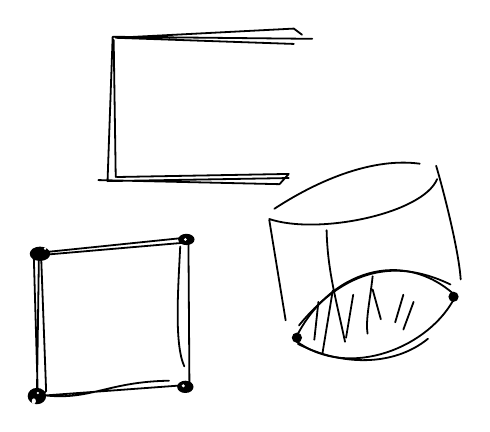
\begin{tikzpicture}[x=.013cm,y=-.013cm,line width=.65pt,line cap=round,line join=round]
\draw (1805,608)--(1610,606)--(1605,747)--(1782,744)
 (1795,604)--(1787,598)--(1613,607)--(1787,613)
 (1611,609)--(1613,743) (1596,746)--(1773,750)--(1782,740)--(1614,743);
\draw (1538,817)--(1684,802)--(1685,946)--(1536,957)--cycle
 (1543,819)--(1682,807) (1533,822)--(1537,960)--(1545,952)--(1540,817)
 (1676,811)..controls(1674,852)and(1670,906)..(1680,928)
 (1541,956)..controls(1588,962)and(1604,943)..(1665,942);
% Mostly black corner knots with small off-centre white counters.
\fill (1539,818) ellipse[x radius=10,y radius=7]
 (1682,804) ellipse[x radius=8,y radius=5.5]
 (1681,948) ellipse[x radius=8,y radius=6]
 (1536,957) ellipse[x radius=9,y radius=8];
\fill[white] (1544,813) circle[radius=1.3]
 (1681,804) circle[radius=1.5] (1679,947) circle[radius=1.6]
 (1537,954) circle[radius=1.2];
\fill[white] (1533,962) ellipse[x radius=2,y radius=2.8];
\draw (1768,774)..controls(1814,744)and(1866,724)..(1910,730)
 (1763,784)..controls(1810,800)and(1913,779)..(1927,745)
 (1763,785)--(1779,883) (1926,732)..controls(1932,752)and(1948,813)..(1950,843)
 (1819,795)..controls(1820,835)and(1828,861)..(1837,904);
\draw (1789,900)..controls(1822,834)and(1894,812)..(1945,859)
 ..controls(1921,909)and(1841,942)..(1789,903);
\draw (1792,888)..controls(1832,839)and(1880,819)..(1940,848)
 (1791,906)..controls(1834,928)and(1885,928)..(1918,901);
\draw (1811,865)--(1807,902) (1825,854)--(1815,915) (1845,858)--(1838,900)
 (1864,840)..controls(1861,866)and(1857,883)..(1859,896)
 (1864,853)--(1872,882) (1894,858)--(1886,885) (1904,865)--(1894,892);
\fill (1790,900) circle[radius=5] (1943,860) circle[radius=5];
\end{tikzpicture}}

\[
\tikz[x=.014cm,y=-.014cm,baseline=(xone.base)]{
 \node[inner sep=0pt] (xzero) at (420,966) {\(\unsure{X_0|X_{\varnothing}}\)};
 \node[inner sep=0pt] (xone) at (544,953) {\(X_1\)};
 \draw[line width=.32pt] (437,994)..controls(467,976)and(489,944)..(508,952)
 ..controls(525,957)and(511,982)..(534,981)
 ..controls(551,978)and(565,959)..(580,958)--(584,972);
 \fill (506,920) circle[radius=1.4]; % detached ink fleck, no inferred accent
}
\]

\[
\bullet\quad O_1\subset\mathbb F_1\qquad
\deleted{\mathbb F}O_2\subset\mathbb F_2\quad\text{---}\quad O_n\subset\mathbb F_n
\]

\[
% The overlay is certain; which letter was written last is not.
\unsure{\deleted{O}\hat{\mathbb F}|\deleted{\mathbb F}\hat O}\subset\mathbb F
\]

\[
\mathbb F_1\times\text{---}\ \times\mathbb F_n\times(-\,?)
\]

\[
(O_1,\mathbb F_1)\mathbin{*}(O_2,\mathbb F_2)\ \text{---}\mathbin{*}
(\deleted{\unsure{O|0}}\unsure{O_3|O_n}\,\unsure{F_n|F_{n+1}|F_3})\,.
\]

\figure{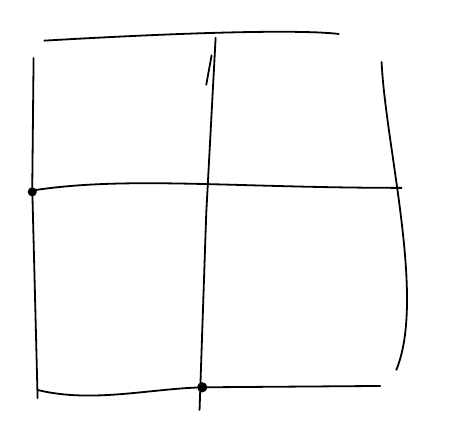
\begin{tikzpicture}[x=.017cm,y=-.017cm,line width=.65pt,line cap=round]
\draw (1374,1202)..controls(1460,1197)and(1559,1193)..(1594,1197)
 (1366,1215)--(1365,1312)--(1369,1469)
 (1365,1314)..controls(1435,1303)and(1515,1312)..(1641,1312)
 (1502,1200)--(1495,1331)--(1490,1478)
 (1499,1213)--(1495,1235)
 (1369,1463)..controls(1410,1473)and(1452,1462)..(1493,1461)--(1625,1460)
 (1626,1218)..controls(1629,1281)and(1659,1395)..(1637,1448);
\fill (1365,1315) circle[radius=3.4] (1492,1461) circle[radius=3.8];
\end{tikzpicture}}

\[
% The final overlaid sign follows the first candidate of the inclusion above.
(F\times I)\mathbin{\amalg}_{\unsure{\deleted{O}\dot{\mathbb F}|\dot B}\times I}
\deleted{O}\hat{\mathbb F}
\]
% archive sheet number: 3
